% ============================================================================
% MedConnect: Clinic Appointment Management System
% Final Database Design & Application Submission | Group-11 | P2 Section
% ============================================================================
\documentclass[10pt,a4paper]{article}
\usepackage[margin=1.75cm,headheight=15pt,footskip=24pt]{geometry}
\usepackage[T1]{fontenc}
\usepackage[utf8]{inputenc}
\usepackage{lmodern,microtype,graphicx,xcolor,titlesec,enumitem,booktabs,tabularx,array,fancyhdr,amsmath,tikz}
\usepackage[hidelinks]{hyperref}
\usetikzlibrary{positioning,arrows.meta,calc}
\definecolor{primaryblue}{HTML}{1A3C6E}
\definecolor{accentblue}{HTML}{2E6DA4}
\definecolor{teal}{HTML}{167B74}
\definecolor{pale}{HTML}{F0F5F8}
\definecolor{graytext}{HTML}{566675}
\hypersetup{pdftitle={MedConnect: Final Database Design and Application},pdfauthor={Group-11}}
\pagestyle{fancy}\fancyhf{}
\fancyhead[L]{\small\color{graytext}MedConnect --- Final Submission}
\fancyhead[R]{\small\color{graytext}Group-11 $|$ DBMS Project}
\fancyfoot[C]{\small\thepage}
\renewcommand{\headrulewidth}{0.3pt}
\titleformat{\section}{\large\bfseries\color{primaryblue}}{\thesection.}{.5em}{}[\vspace{.15em}\color{accentblue}\titlerule]
\titleformat{\subsection}{\normalsize\bfseries\color{accentblue}}{}{0pt}{}
\titlespacing{\section}{0pt}{0pt}{11pt}
\titlespacing{\subsection}{0pt}{10pt}{5pt}
\setlist[itemize]{leftmargin=15pt,itemsep=3pt,topsep=3pt}
\setlist[enumerate]{leftmargin=16pt,itemsep=4pt,topsep=3pt}
\setlength{\parindent}{0pt}\setlength{\parskip}{5pt}
\renewcommand{\arraystretch}{1.22}
\newcommand{\rel}[2]{\par\noindent\textbf{\color{primaryblue}#1}\par\nobreak{\footnotesize\ttfamily\raggedright #2\par}\vspace{1pt}}
\newcommand{\pk}[1]{\underline{#1}}

\begin{document}
\begin{center}
{\LARGE\bfseries\color{primaryblue}MedConnect: Clinic Appointment\\Management System}\par
\vspace{4pt}{\color{graytext}Final Database Design \& Application Submission}\par
{\small Group-11 $|$ P2 Section $|$ November 2026}\par\vspace{4pt}
\begin{tabular}{ll}
\textbf{2022A7PS0059H} & Charan Teja Valavala\\
\textbf{2023A3PS0304H} & Rithwik Sai Madadi\\
\textbf{2023A3PS0325H} & Peketi Sai Manoj\\
\textbf{2023A3PS0367H} & Y Sameeksha\\
\textbf{2023A3PS0368H} & K S Rajeev Kasyap
\end{tabular}
\end{center}
\vspace{5pt}
\section{Problem Statement, Scope \& Application Design}
\textbf{Objective.} Integrate patient registration, provider schedules, appointment booking, clinical encounters, pharmacy dispensing, billing, and reporting for a multi-specialty outpatient clinic. The database remains the core: the application exercises ten related tables through parameterized SQL and transactional workflows.

\subsection{Intended Users \& Assumptions}
\begin{itemize}
\item \textbf{Admin/Receptionist:} maintains patient entries, books/reschedules/cancels visits, manages the medicine catalog and stock receipts, records payments, and reads clinic reports.
\item \textbf{Doctor:} views assigned appointments and relevant patient records, starts consultations, and completes clinical notes and prescriptions. Patients are data entities; there is no patient login.
\item One doctor belongs to one department. Shifts recur weekly, within one day; the clinic uses Asia/Kolkata time and INR. Appointment duration is captured from its shift.
\item A visit has at most one medical record, prescription header, and invoice. A prescription can contain multiple distinct medicines. Historical records may have a null appointment link.
\item Cancelled bookings remain in history and release their slots. Completed notes, dispenses, and issued invoice amounts cannot be edited through the supported workflows.
\end{itemize}

\subsection{Integrated End-to-End Workflows}
\begin{enumerate}
\item \textbf{Booking \& concurrency:} reception registers/selects a patient, retrieves an active doctor's available times, and books a future visit. Shift checks, a provider row lock, overlap detection, and a partial unique index reject collisions. Cancellation permits rebooking.
\item \textbf{Clinical encounter \& pharmacy:} the assigned doctor starts a visit, records findings, and submits prescription lines. A trigger locks each medicine, rejects expired/insufficient stock, captures the unit price, and deducts quantity. A failure rolls back the entire encounter.
\item \textbf{Billing \& analytics:} encounter completion calls the invoice procedure. Reception records a payment; the paid-only department view and SQL reports reflect the change.
\end{enumerate}

\subsection{Technology Stack \& Architecture}
\begin{center}
\colorbox{pale}{\parbox{.94\linewidth}{\centering\vspace{5pt}
\textbf{React 18 + Vite + Tailwind CSS + TanStack Query}\\[-1pt]
\small Staff/doctor interface, forms, schedule, inventory, reports\\
$\updownarrow$ REST/JSON with bearer authentication\\
\textbf{FastAPI + Pydantic + asyncpg} $\longleftrightarrow$ \textbf{PostgreSQL 16}\\
Raw bound SQL, connection pool, transactions, PL/pgSQL routines\vspace{5pt}}}
\end{center}

\newpage
\section{Final Conceptual ER Model}
Entities have independent surrogate identifiers. Dependent existence alone does not make an entity weak in the identifying-key sense. Prescription--Medicine is an M:N relationship resolved by \texttt{Prescription\_Items}. The diagram shows minimum/maximum participation for the primary links; direct provenance links are listed below and on page 3.
\vspace{6pt}
\begin{center}
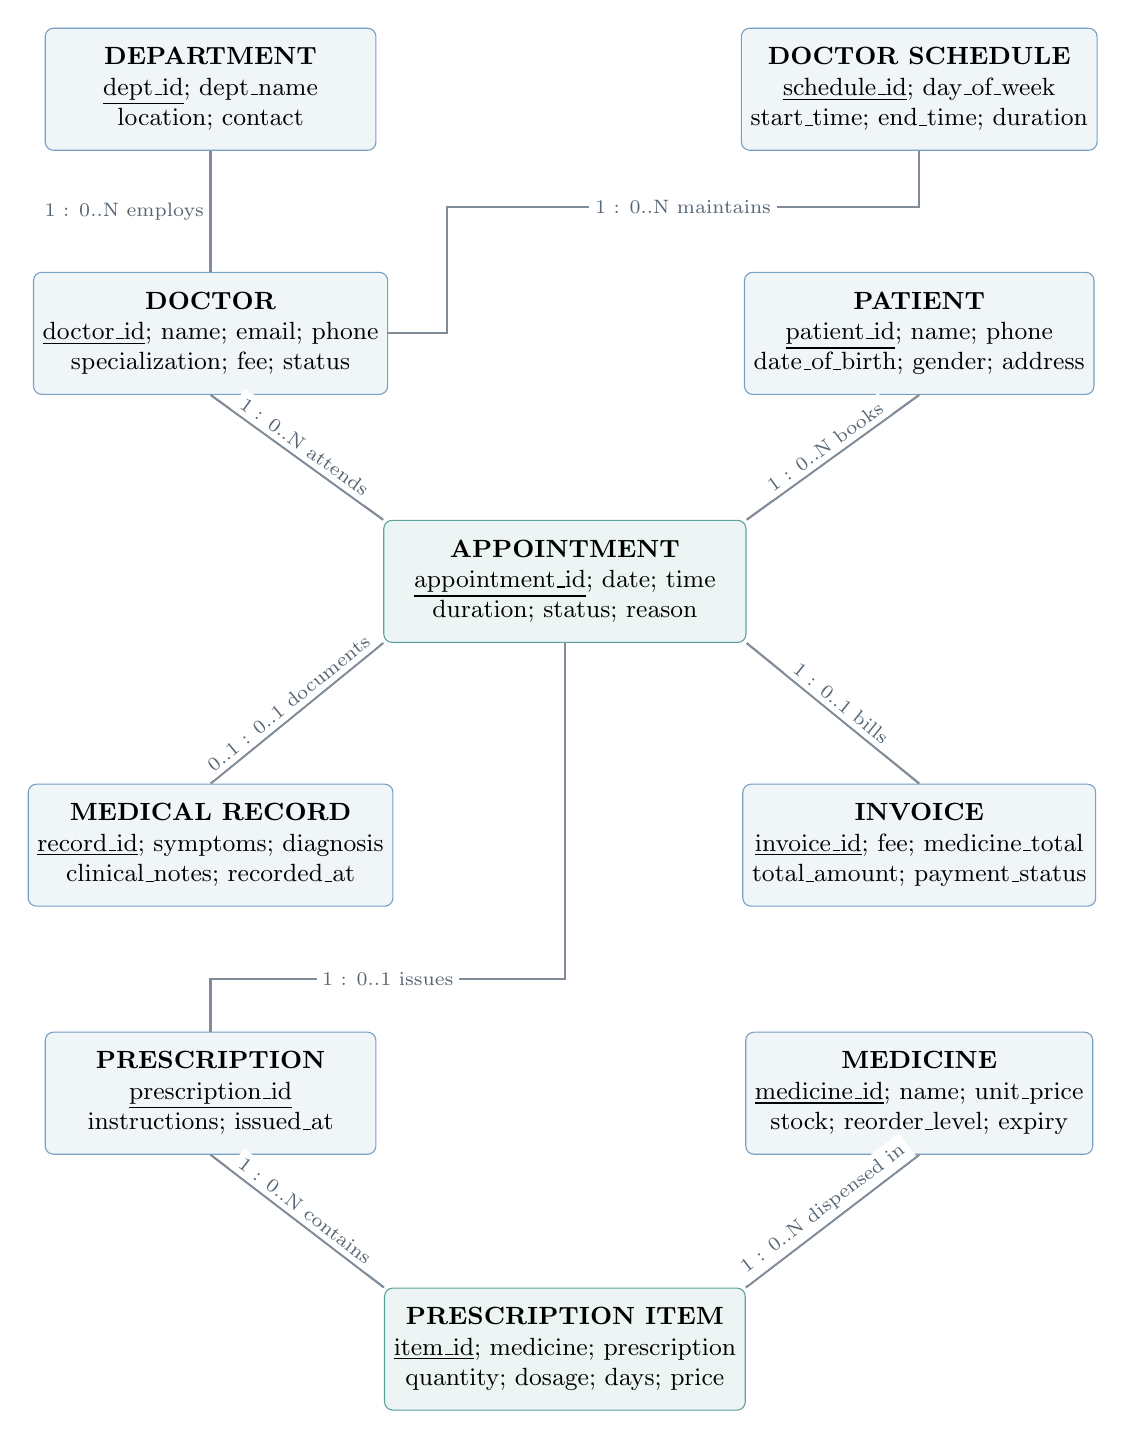
\begin{tikzpicture}[
  entity/.style={draw=accentblue!65,fill=pale,rounded corners=3pt,minimum width=4.2cm,minimum height=1.55cm,align=center,font=\small},
  link/.style={draw=graytext!75,thick},
  cardinal/.style={font=\scriptsize,fill=white,inner sep=2pt,text=graytext}
]
\node[entity] (dept) at (0,0) {\textbf{DEPARTMENT}\\\underline{dept\_id}; dept\_name\\location; contact};
\node[entity] (schedule) at (9,0) {\textbf{DOCTOR SCHEDULE}\\\underline{schedule\_id}; day\_of\_week\\start\_time; end\_time; duration};
\node[entity] (doctor) at (0,-3.1) {\textbf{DOCTOR}\\\underline{doctor\_id}; name; email; phone\\specialization; fee; status};
\node[entity] (patient) at (9,-3.1) {\textbf{PATIENT}\\\underline{patient\_id}; name; phone\\date\_of\_birth; gender; address};
\node[entity,minimum width=4.6cm,fill=teal!8,draw=teal!70] (appt) at (4.5,-6.25) {\textbf{APPOINTMENT}\\\underline{appointment\_id}; date; time\\duration; status; reason};
\node[entity] (record) at (0,-9.6) {\textbf{MEDICAL RECORD}\\\underline{record\_id}; symptoms; diagnosis\\clinical\_notes; recorded\_at};
\node[entity] (invoice) at (9,-9.6) {\textbf{INVOICE}\\\underline{invoice\_id}; fee; medicine\_total\\total\_amount; payment\_status};
\node[entity] (rx) at (0,-12.75) {\textbf{PRESCRIPTION}\\\underline{prescription\_id}\\instructions; issued\_at};
\node[entity] (med) at (9,-12.75) {\textbf{MEDICINE}\\\underline{medicine\_id}; name; unit\_price\\stock; reorder\_level; expiry};
\node[entity,fill=teal!8,draw=teal!70] (items) at (4.5,-16) {\textbf{PRESCRIPTION ITEM}\\\underline{item\_id}; medicine; prescription\\quantity; dosage; days; price};
\draw[link] (dept) -- node[cardinal,left]{1 : 0..N employs} (doctor);
\draw[link] (doctor.east) -- (3,-3.1) -- (3,-1.5) -- (9,-1.5) -- (schedule.south);
\node[cardinal] at (6,-1.5) {1 : 0..N maintains};
\draw[link] (doctor.south) -- node[cardinal,sloped,above]{1 : 0..N attends} (appt.north west);
\draw[link] (patient.south) -- node[cardinal,sloped,above]{1 : 0..N books} (appt.north east);
\draw[link] (appt.south west) -- node[cardinal,sloped,above]{0..1 : 0..1 documents} (record.north);
\draw[link] (appt.south east) -- node[cardinal,sloped,above]{1 : 0..1 bills} (invoice.north);
\draw[link] (appt.south) -- (4.5,-11.3) -- (0,-11.3) -- (rx.north);
\node[cardinal] at (2.25,-11.3) {1 : 0..1 issues};
\draw[link] (rx.south) -- node[cardinal,sloped,above]{1 : 0..N contains} (items.north west);
\draw[link] (med.south) -- node[cardinal,sloped,above]{1 : 0..N dispensed in} (items.north east);
\end{tikzpicture}
\end{center}
\vspace{2pt}
{\small\textbf{Provenance links.} Each record and prescription references exactly one patient and doctor; each invoice references one patient. Linked identities must match the appointment. Records may exist without an appointment for imported history. A header can have zero lines at the relational level; the application only creates a prescription when medicines are selected.}

\newpage
\section{Relational Schema, Keys \& Domains}
\textbf{Notation:} underlined attributes are primary keys; $\ast$ marks foreign keys; $?$ marks nullable attributes. \texttt{created\_at} is a timezone-aware timestamp where listed. All identifier keys are auto-incrementing integers. Full executable DDL is in \texttt{schema.sql}.
\vspace{5pt}
\begingroup\setlength{\parskip}{2pt}
\rel{1. Departments}{(\pk{dept\_id}, dept\_name, description?, location, contact\_number?, created\_at)}
\rel{2. Doctors}{(\pk{doctor\_id}, dept\_id*, first\_name, last\_name, email, phone, specialization, qualification, consultation\_fee, status, password\_hash?, created\_at)}
\rel{3. Doctor\_Schedules}{(\pk{schedule\_id}, doctor\_id*, day\_of\_week, start\_time, end\_time, slot\_duration\_minutes, is\_active)}
\rel{4. Patients}{(\pk{patient\_id}, first\_name, last\_name, date\_of\_birth, gender, blood\_group?, phone, email?, address, emergency\_contact\_phone?, created\_at)}
\rel{5. Appointments}{(\pk{appointment\_id}, patient\_id*, doctor\_id*, appointment\_date, appointment\_time, duration\_minutes, status, reason\_for\_visit?, created\_at)}
\rel{6. Medical\_Records}{(\pk{record\_id}, appointment\_id*?, patient\_id*, doctor\_id*, symptoms, diagnosis, clinical\_notes?, recorded\_at)}
\rel{7. Prescriptions}{(\pk{prescription\_id}, appointment\_id*, patient\_id*, doctor\_id*, instructions?, issued\_at)}
\rel{8. Medicines}{(\pk{medicine\_id}, name, category, manufacturer, unit\_price, stock\_quantity, reorder\_level, expiry\_date, created\_at)}
\rel{9. Prescription\_Items}{(\pk{item\_id}, prescription\_id*, medicine\_id*, dosage, duration\_days, quantity, unit\_price)}
\rel{10. Invoices}{(\pk{invoice\_id}, appointment\_id*, patient\_id*, consultation\_fee, medicine\_total, total\_amount, payment\_status, payment\_method?, issued\_at, paid\_at?)}
\endgroup

\subsection{Foreign Keys \& Referential Actions}
{\small
\begin{tabularx}{\linewidth}{@{}p{3.0cm}X p{2.1cm}@{}}
\toprule \textbf{Child relation} & \textbf{Referenced parent(s)} & \textbf{On delete}\\\midrule
Doctors & Departments & RESTRICT\\
Doctor\_Schedules & Doctors & CASCADE\\
Appointments & Patients; Doctors & RESTRICT\\
Medical\_Records & Appointments; Patients; Doctors & SET NULL; RESTRICT\\
Prescriptions & Appointments; Patients; Doctors & RESTRICT\\
Prescription\_Items & Prescriptions; Medicines & CASCADE; RESTRICT\\
Invoices & Appointments; Patients & RESTRICT\\\bottomrule
\end{tabularx}}
{\small The DDL retains these referential actions from the mid-sem model; final retention triggers additionally block deleting appointments, schedules, clinical records, prescriptions, dispenses, and invoices. Cascades therefore do not provide a supported way to erase clinical history.}

\subsection{Candidate Keys \& Attribute Domains}
{\small \textbf{Unique:} department name; doctor email and phone; patient phone and non-null email (within their respective tables); medicine name; (doctor, weekday, shift start); (prescription, medicine); non-null appointment in records; appointment in prescriptions and invoices. Money uses \texttt{NUMERIC(10,2)}; stock/quantity are integers; visit dates use \texttt{DATE}; local slots use \texttt{TIME}; event timestamps use \texttt{TIMESTAMPTZ}. Names/contact fields use bounded strings and clinical notes use \texttt{TEXT}.}

\newpage
\section{Integrity Constraints, Transactions \& Normalization}
\subsection{Database-Enforced Rules}
{\small
\begin{tabularx}{\linewidth}{@{}p{3.0cm}X@{}}
\toprule \textbf{Rule} & \textbf{Enforcement and outcome}\\\midrule
Identity and existence & Ten primary keys and foreign keys preserve references. Clinical-link triggers reject patient/doctor mismatches; invoice identity must match the completed visit.\\
Domains and arithmetic & CHECK validates allowed statuses, positive quantities/days, nonnegative prices/stock/fees, ordered shift times, and invoice total = consultation fee + medicine total.\\
Booking availability & Active provider; matching weekday shift; exact slot alignment; duration snapshot; provider row lock; overlap check. The partial unique index excludes only Cancelled rows.\\
Lifecycle and retention & Scheduled $\to$ In\_Consultation $\to$ Completed, or Scheduled $\to$ Cancelled/No\_Show. A clinical record is required for completion. Only Scheduled visits can move. Historical/clinical deletes and edits are rejected.\\
Pharmacy & BEFORE INSERT trigger locks the medicine, checks expiry/stock, snapshots its price, and deducts quantity. Duplicate medicine lines are unique per prescription. Dispenses are retained.\\
Billing and payment & Procedure locks the appointment, requires Completed, sums dispensed price snapshots, and returns on a repeated call. Insert trigger checks fee/medicine amounts. Issued amounts are fixed; supported payment transition is Pending $\to$ Paid.\\\bottomrule
\end{tabularx}}

\subsection{Transaction Boundaries \& Concurrency}
The backend uses \texttt{asyncpg} transactions at PostgreSQL's default READ COMMITTED isolation. Completion writes the medical record, prescription and lines, stock changes, status, and invoice in one transaction. Any invalid medicine aborts all of them. Item locks are acquired in medicine-ID order. Invoice generation and payment serialize on their parent rows; repeating payment with the same method returns the existing result.

The availability list is advisory: a competing booking can win before confirmation. The database rechecks the write; the API returns HTTP 409 and the interface offers refreshed times. Row locks preserve stock under competing prescriptions, rather than relying on the frontend's displayed quantity.

\subsection{Normalization \& Deliberate Redundancy}
\begin{itemize}
\item \textbf{1NF:} atomic attributes, with medication lines in a separate relation. The history report builds JSON at query time; it is not stored as repeating groups.
\item \textbf{2NF/3NF:} catalog, department, patient, provider, and schedule facts are separated. Prescription-item attributes depend on the whole (prescription, medicine) key. Department descriptions are not repeated in doctor rows.
\item \textbf{BCNF under the stated dependencies:} master/schedule/appointment/item relations use superkey determinants. A nullable UNIQUE appointment link in records is not an unconditional relational candidate key; multiple legacy rows may have null links.
\item \textbf{Controlled redundancy:} linked clinical headers repeat patient/doctor IDs for provenance, enforced by triggers. Invoice patient is derived from its unique appointment. \texttt{total\_amount} is stored for billing, despite the non-key dependency (consultation fee, medicine total) $\to$ total. Thus a universal BCNF claim is not made. A CHECK maintains this arithmetic.
\item \textbf{Historical prices:} dispensed unit price and issued consultation fee are time-specific facts, independent of later catalog changes. They prevent retroactive repricing.
\end{itemize}
\textbf{Temporal validation.} Stable domain checks remain in DDL. The API validates future birth dates and past bookings; dispensing expiry is checked at write time. PostgreSQL assumes CHECK conditions remain valid for the same row values, so cross-row and time-sensitive workflow rules belong in triggers/application validation.

\newpage
\section{SQL Evidence, Final Decisions \& Team Responsibilities}
\subsection{Five Executable Reports \& Additional DBMS Features}
{\small
\begin{tabularx}{\linewidth}{@{}>{\raggedright\arraybackslash\footnotesize}p{3.8cm}>{\raggedright\arraybackslash}X@{}}
\toprule \textbf{SQL report in database/queries} & \textbf{Purpose and concepts exercised}\\\midrule
01\_department\_revenue.sql & Current-month billed, collected, and pending amounts by specialty; joins, CTE, filtered aggregates, DENSE\_RANK, and SUM OVER.\\
02\_doctor\_performance.sql & Last-30-day completed/cancelled/no-show counts, attendance and collections; outer joins, grouping, FILTER and NULLIF.\\
03\_pharmacy\_reorder.sql & Low/expired stock, recent dispensing velocity and estimated days remaining; two CTEs, joins, CASE and guarded division.\\
04\_patient\_history.sql & Patient encounters and dispensed medication snapshots; multi-table joins, correlated subquery, ordered JSON aggregation; bound patient/doctor parameters.\\
05\_peak\_demand.sql & Last-90-day visits by weekday/hour and no-show rate; date extraction, grouped CTE, filtered counts and RANK.\\\bottomrule
\end{tabularx}}
\textbf{Additional features:} explicit transactions and row locks; PL/pgSQL triggers; stored invoice procedure; paid-only department revenue view; partial unique and query-supporting B-tree indexes. Their use follows the three workflows rather than adding unrelated objects.

\subsection{Important Final Design Decisions}
\begin{enumerate}
\item Retain the ten-table mid-sem scope and raw SQL stack. Add doctor password hashes, appointment duration, and dispensed unit-price snapshots without an extra account table. The administration identity is configured outside the database.
\item Treat doctors and administration as distinct application roles. Signed, expiring tokens and PBKDF2 password hashes protect staff access; doctor reads are scoped to assigned encounters. No patient self-service, insurance adjudication, refunds, split payments, or multi-clinic operation is implemented.
\item Preserve clinical and billing history. Corrections/refunds would need a separate, designed amendment workflow; issued records are not silently overwritten.
\item Keep reproducibility explicit: schema, synthetic seed script, environment generator, dependency locks, Docker Compose, native instructions, and PostgreSQL-backed tests. Lists are bounded for the lab demonstration; the reports query the underlying relations directly.
\end{enumerate}

\subsection{Group-11: Continued Roles \& Final Module Responsibilities}
{\small
\begin{tabularx}{\linewidth}{@{}p{3.05cm}p{2.65cm}X@{}}
\toprule \textbf{Member} & \textbf{BITS ID} & \textbf{Responsibility}\\\midrule
K S Rajeev Kasyap & 2023A3PS0368H & ER/relational diagrams, schema, keys, indexes, schedule and booking design.\\
Rithwik Sai Madadi & 2023A3PS0304H & Backend/database integration, patient and booking APIs, staff access, setup.\\
Peketi Sai Manoj & 2023A3PS0325H & Clinical integrity, stock trigger, invoice procedure, concurrency, normalization.\\
Y Sameeksha & 2023A3PS0367H & React interface, staff/doctor workflows, validation, responsive layout, demo.\\
Charan Teja Valavala & 2022A7PS0059H & SQL reports, sample-data/verification coordination, final report, README, viva preparation.\\\bottomrule
\end{tabularx}}
{\small These responsibilities continue the submitted mid-sem roles. Every member must understand the entire relational design and reproduce the integrated workflows for the individual viva.}

\subsection{Reproduction \& Verification Route}
{\small Run \texttt{scripts/setup\_env.py}, then follow the native or Compose route in README. A fresh seed creates \textbf{1,308 synthetic records} across ten relations. \texttt{scripts/verify\_db.py} runs all five reports. PostgreSQL tests cover keys/domains, slot races, stock races, rollback, pricing, invoice retries, permissions, and HTTP workflows. \texttt{docs/demo\_guide.md} gives the live-demo sequence; \texttt{docs/verification.md} records verified results and limits.}

{\footnotesize\color{graytext}\textbf{References:} DBMS Project Guidelines, Sections 3--8; PostgreSQL 16 documentation, Sections 5.4 (constraints), 11.8 (partial indexes), and 13.3 (explicit locking). Repository: \url{https://github.com/charanvalavala/medconnect-final-submission}.}
\end{document}
